Little introduction: 
\begin{itemize}
    \item Experimental and theoretical physicist, was the old distinction
    \item The different categories of astronomy
    \item The uniqueness of a computational astrophysicist
    \item What is the job of a computational astrophysicist
    \item How a computational astrophysicist is doing a “theoretical experiment”
    \item How this thesis fits in that 
\end{itemize}


\section{The Explicit Physics}
    My simulations solve the \textit{restricted three body problem}. In essence
    \begin{figure}
        \centering
        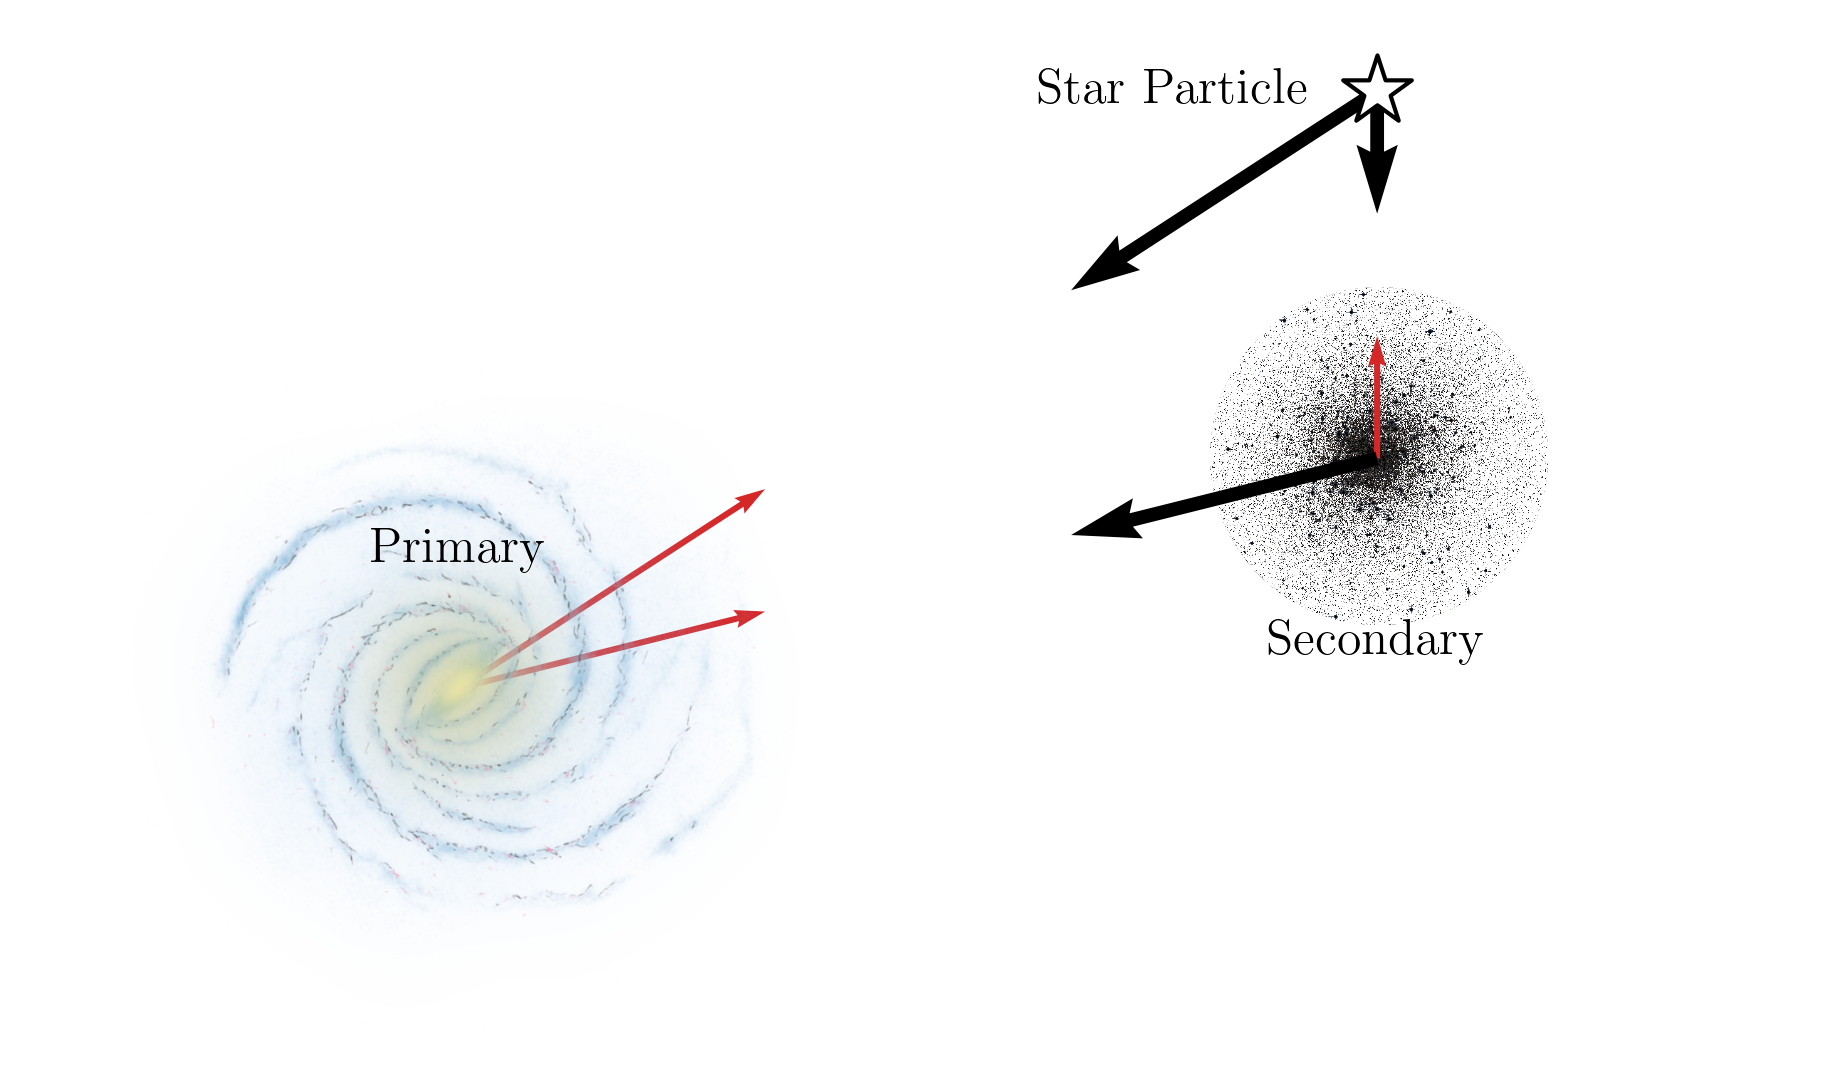
\includegraphics[width=\linewidth]{images/restricted_three_body_set_up.png}
        \caption{Little sketch of my equations of motion. }
    \end{figure}
    
    \subsection{Equations of Motion} \label{subsec:myEquationsOfMotion}
        I like to start with the \textit{Lagrangian}, which comes from the variational principle which states that particles with move along trajectories that minimize the difference, $ L = T-U $, which $L$ is the Lagrangian, $T$ is the kinetic energy and $U$ is the potential energy. Also, as is almost always the case in gravitational dynamics, we normalize by the mass and use \textit{specific} energy: 
        \begin{equation}
            \mathcal{L} = \frac{L}{m} = \frac{1}{2}\left(\dot{x}^2+\dot{y}^2+\dot{z}^2\right) - \Phi(x,y,z).
        \end{equation}
        However, Lagrange's equations give a system of three second order coupled ordinary differential equations. If we switch to Hamiltonain dynamics, we can object a set of six \textit{first} order ordinary differential equations, which is easier to implement computationally. Also, since we are using the specific energy, the momentum coordinates for Hamilton's equations are the same as the velocities from the Lagrangian: $ p_i = \frac{\partial \mathcal{L}}{\partial \dot{q}_i}$. Therefore, $p_i = \dot{q}_i$, where $i \in \left(x,y,z\right)$. The Hamilton is derived through the Legendre transform: $ \mathcal{H}=\sum_i p_i\dot{q}_i - \mathcal{L}$. Then, we can apply Hamilton's equations to obtain the set of equations: 
        \begin{align}
            \dot{p}_i &= -\frac{\partial \mathcal{H}}{\partial q_i} \\
            \dot{q}_i &= \frac{\partial \mathcal{H}}{\partial p_i}
        \end{align}

        And when written explicity become: 
        \begin{align}
            \dot{p}_x &= -\frac{\partial \Phi}{\partial x} \\
            \dot{p}_y &= -\frac{\partial \Phi}{\partial y} \\
            \dot{p}_z &= -\frac{\partial \Phi}{\partial z} \\
            \dot{x} &= p_x \\ 
            \dot{y} &= p_y \\ 
            \dot{z} &= p_z \\ 
        \end{align}        




        \subsubsection*{The Globular Cluster}
            hello

        \subsubsection*{The Star Particles}

    \subsection{Potential density pairs}

        \begin{figure}
            \centering
            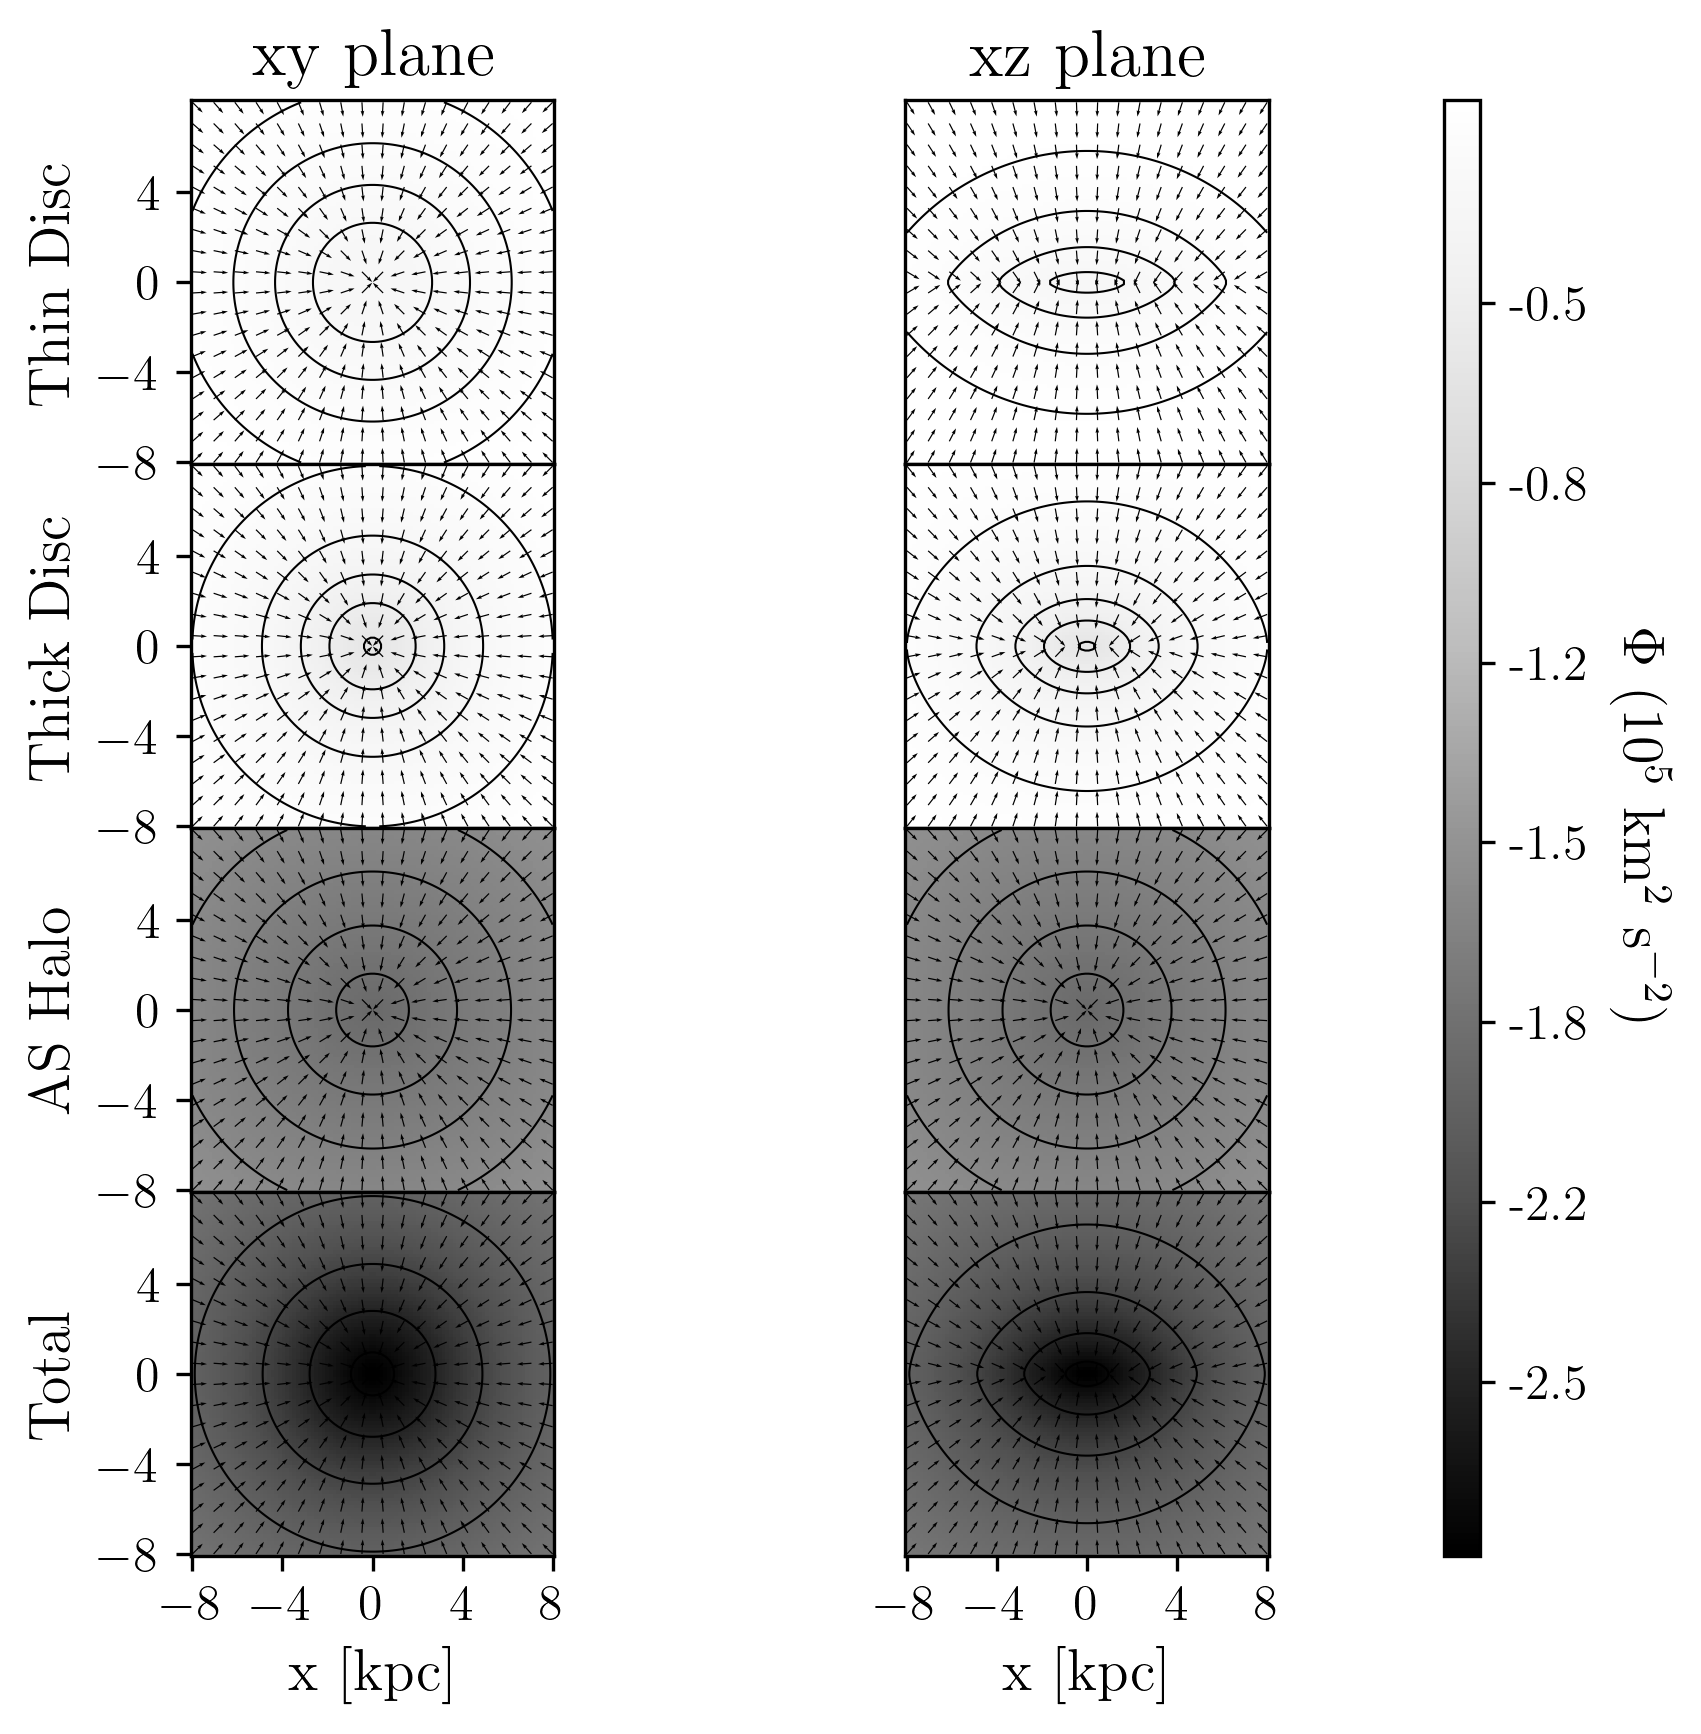
\includegraphics[width=\linewidth]{images/figure_pouliasis2017pii_potential_-8_8.png}
            \caption{The main potential used throughought the thesis}
        \end{figure}        
    

\section{The Implicit Physics}

    \subsection{The circular restricted three body problem}

    \subsection{The tidal tensor}
        
\begin{verbatim}
VIDEO: moon_tidal_simulation.mp4
\end{verbatim}

        \begin{figure}
            \centering
            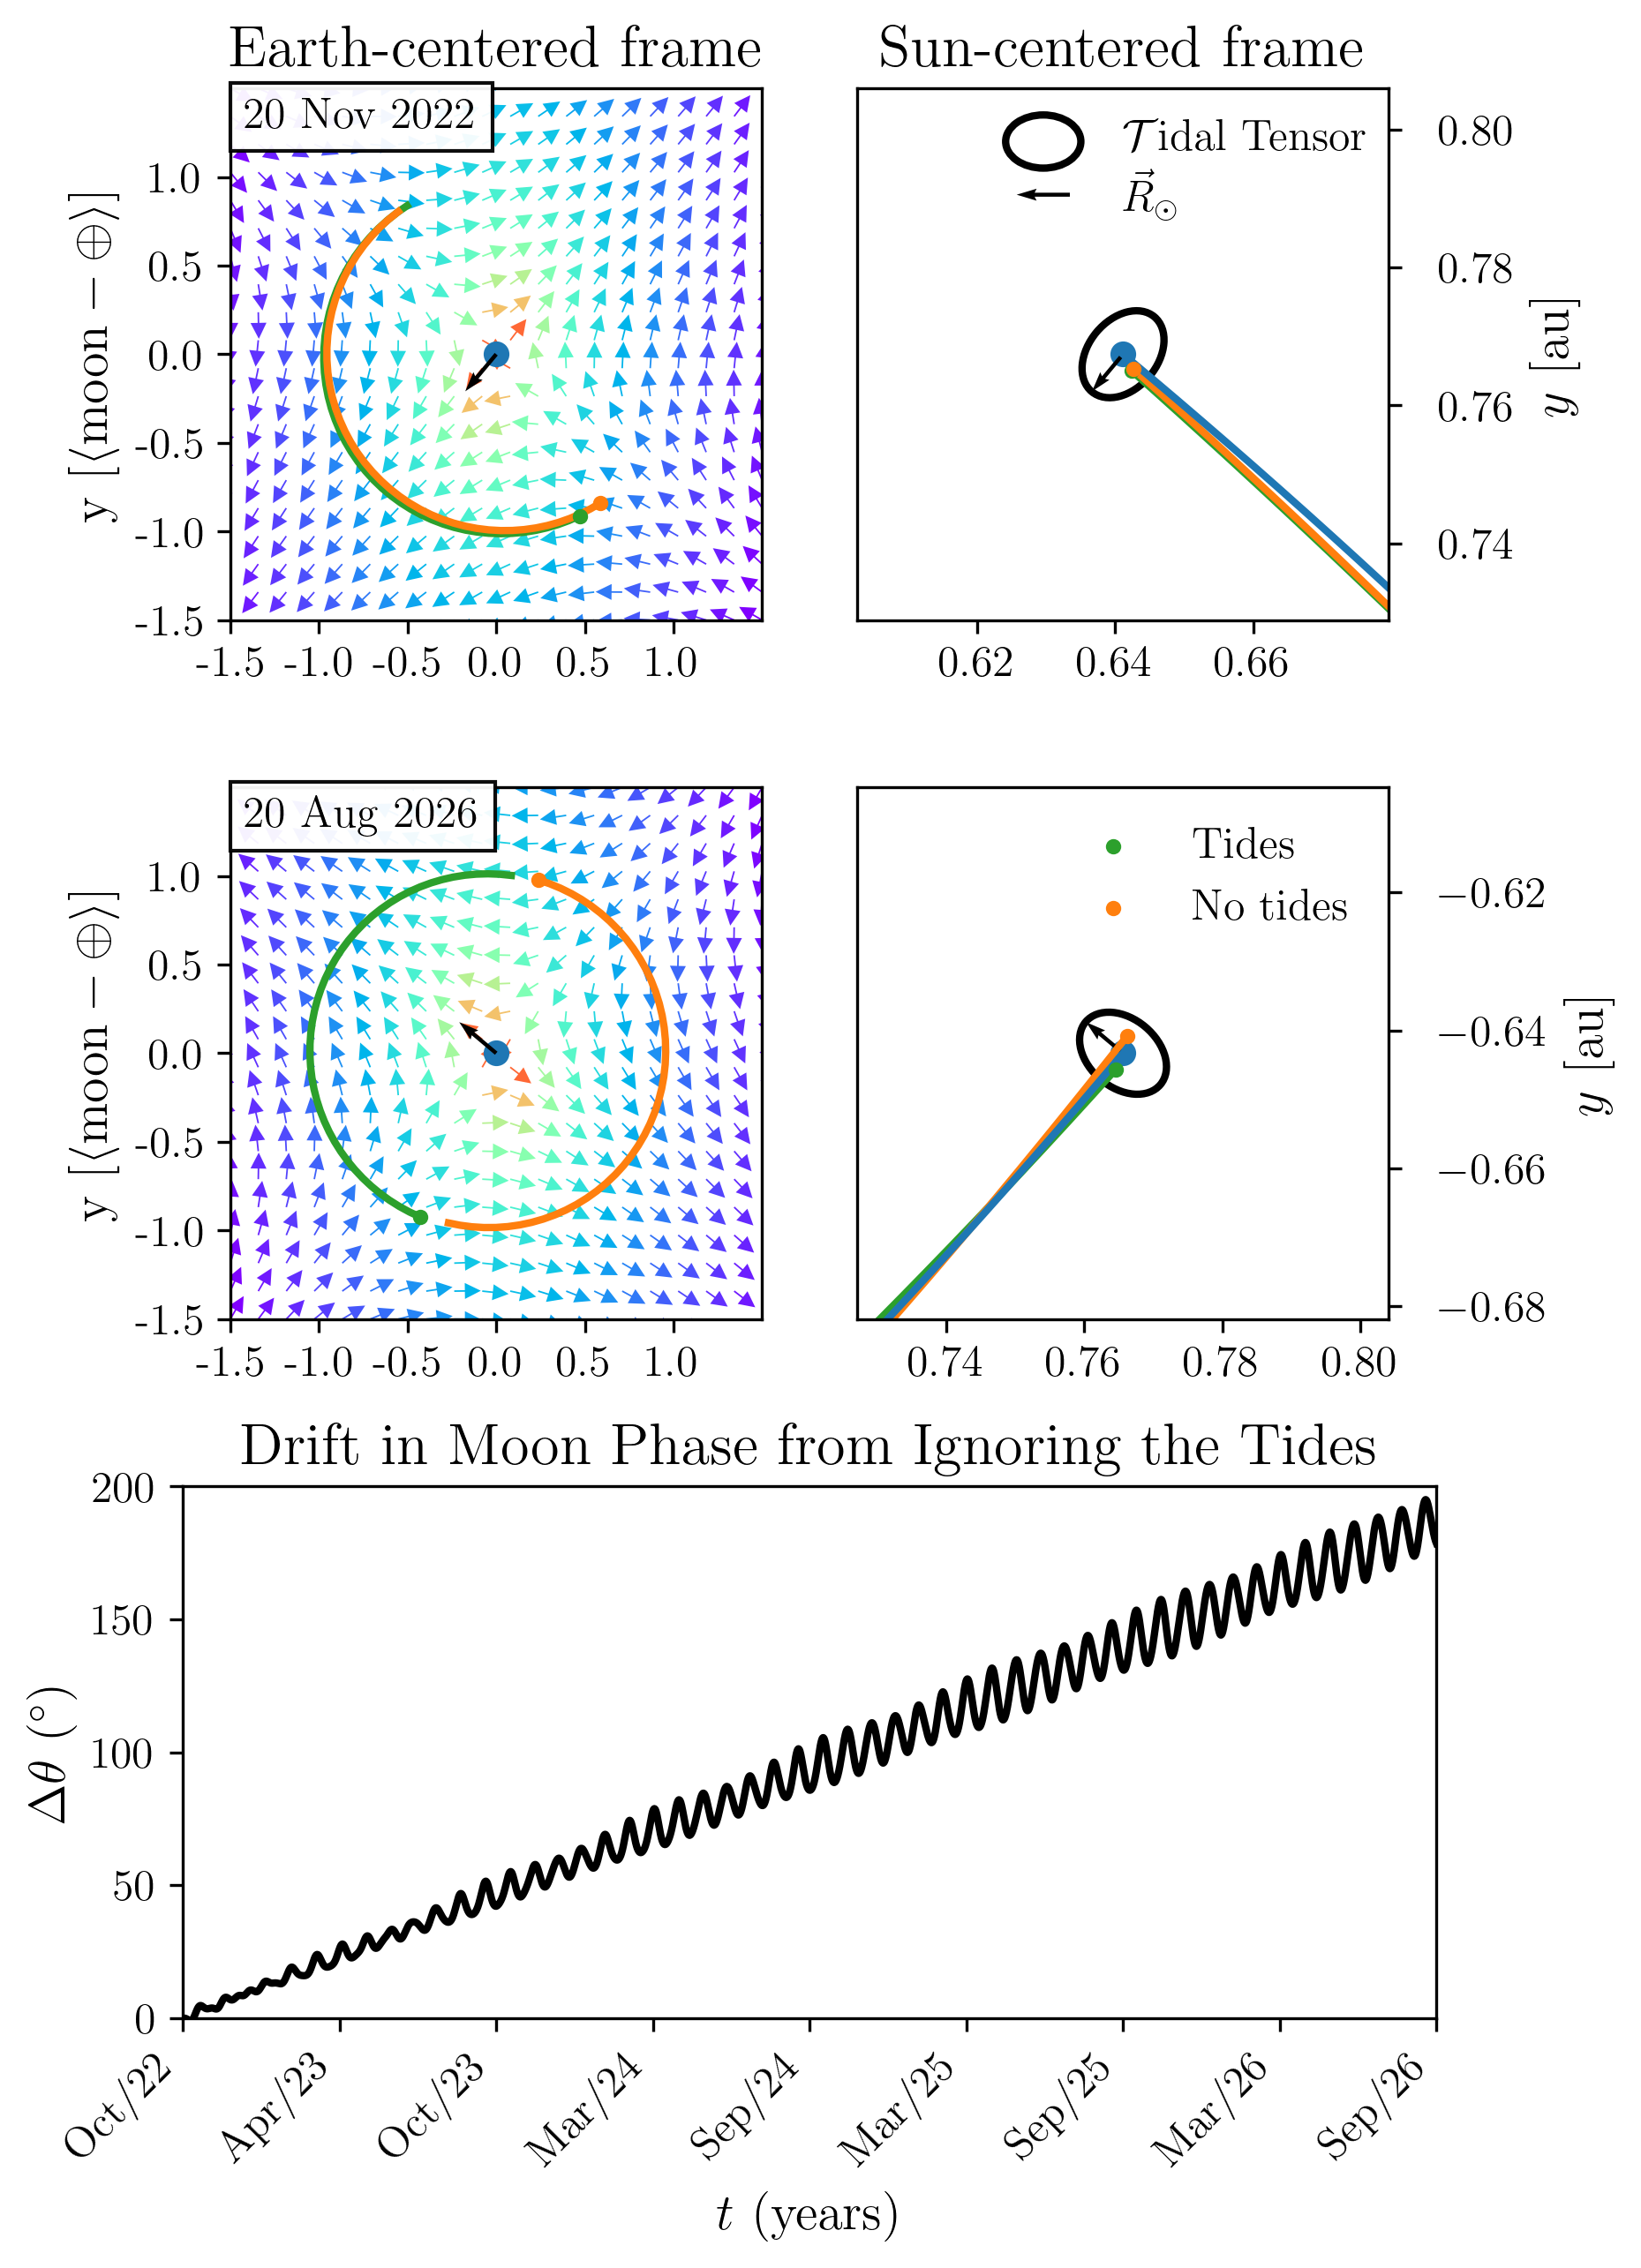
\includegraphics[width=\linewidth]{images/moon_tidal_simulation.png}
            \caption{The main potential used throughought the thesis}
        \end{figure}

        \begin{itemize}
            \item Show the motivating example of the moon. 
            \item Show the tidal tensor moving around in the case of our galactic potential model 
        \end{itemize}


    \subsection{Phase mixing}
        \begin{itemize}
            \item The Luiville theorem
            \item How it is slower with tidal tails 
            \item also the monte-carlo approach with phase mixing is what causes vast differences in orbital solutions after a certain period of time 
        \end{itemize}
    
    \subsection{Shocks}
        I started this section with the circular and planar restricted three body problem. It really simplifies the problem instead of looking for a general solution. All three bodies are point masses, in fact the tertiary body has no mass. The secondary is on a circular orbit about the primary, and the tertiary is in the same orbital plane as the secondary. This simplified problem is already quite complex but solvable and rich with physics. However, by restricting the orbits of the tertiary and secondary, we lose a lot of physics that affects our system. Additionally, for the globular clustres, most of them are not on circular orbits. Additionally, the galaxy is not a point mass, but rather a mass distribution with cylindrical symmetry.        



\section{The Ignored Physics}
    \subsection{Collisional dynamics}
        \begin{itemize}
            \item not nbody
            \item no mass segregation
            \item no three body encounters 
            \item no soft or hard binaries 
            \item show some results from Corespray 
        \end{itemize}
    
    \subsection{Stellar evolution}
        \begin{itemize}
            \item They're all point masses 
            \item No salpeter's 
            \item No strong initial mass loss 
            \item No accurate model for the colors 
            \item No multiple stellar populations 
        \end{itemize}
    
    \subsection{Time evolution}
        In someways, we take time evolution into account, and in someways, we ignore and this has already been covered in the previous sections. i.e., the orbit of the star-particles depend on the position of the host globular cluster, which I do not solve for simoltaneously but instead opt to load it into the computation, as shown in Section~\ref{subsec:myEquationsOfMotion}. Also, things like mass segregation and stellar evolution are time-dependent which is completely ignored in my simulations. 

